\onecolumn
\section{Project Team and Roles}

\begin{IEEEbiography}
[{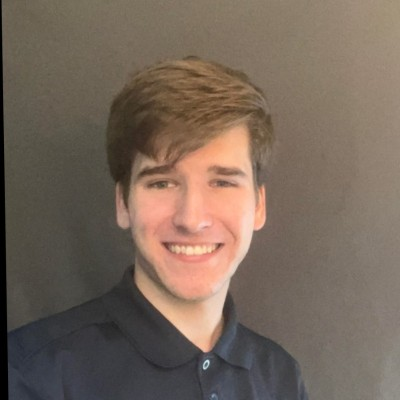
\includegraphics[width=1in,height=1.25in,clip,keepaspectratio]{Headshots/NHeadshot.jpg}}]
{\normalsize Nicholas Krupa}
\normalsize
is a senior electrical engineering major with minors in physics and mathematics. He is the founder and president of the AURORA Rocketry Team, a Senior Research Assistant within the Multiscale Metamaterial Research Laboratory, and holds a Level 2 High Power Rocketry certification through the National Association of Rocketry. He is a recipient of both a NASA Connecticut Space Grant Consortium Undergraduate Scholarship and an Undergraduate Research Grant for his work on phased-array antennas for satellite and space communication \cite{ctsgcSpring2024,ctsgcFall2024}. He is also a co-author of published research involving microwave metasurface design and characterization \cite{wells2024}. For this project, he will coordinate the overall \ares{} mission, including vehicle requirements, subsystem integration, flight operations, and development of the \deimos{} telemetry system and \comet{} flight computer. His previous experience includes leading the University of Hartford NASA RockSat-C team and developing several generations of custom high-power rocketry avionics. He completed an engineering internship with Ensign-Bickford Aerospace \& Defense (EBAD) during Summer 2026 and has accepted a full-time return offer with the company following graduation.
\end{IEEEbiography}

\begin{IEEEbiography}
[{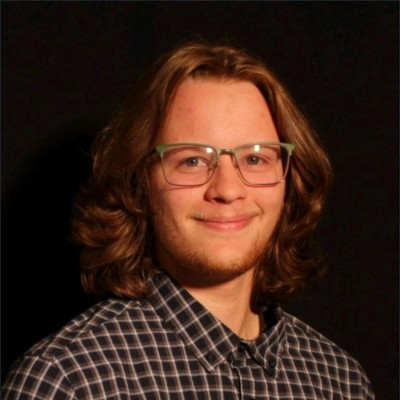
\includegraphics[width=1in,height=1.25in,clip,keepaspectratio]{Headshots/KHeadshot.jpg}}]
{\normalsize Kyle Eckert}

\normalsize
is a senior electrical engineering major with minors in audio engineering and mathematics and serves as the electrical lead for the Multiscale Metamaterial Research Laboratory. His work in the laboratory focuses on the design and development of experimental instrumentation for characterizing material properties at microwave frequencies. He also designs modifications to existing measurement systems to expand their operational and measurement capabilities. He was awarded a NASA Connecticut Space Grant Consortium Undergraduate Research Grant during the Spring 2026 award cycle for research involving rocket-based RF and metamaterial communication systems \cite{ctsgc2026}. Kyle was also the Lead Electrical Engineer and Flight Engineer with the 2026 RockSat program, where he designed and developed circuitry to enable experiments to fly aboard NASA sounding rockets and collect data under flight conditions. He holds a Level 1 High Power Rocketry certification and is a co-creator of the \comet{} dual-deployment system, a four-layer PCB-based avionics system. He will lead the design, fabrication, and testing of the \phobos{} phased-array antenna payload, with emphasis on RF electronics, antenna systems, and communication engineering.
\end{IEEEbiography}



\begin{IEEEbiography}
[{
\includegraphics[width=1in,height=1.25in,clip,keepaspectratio]{Headshots/LHeadshot.jpg}}]
{\normalsize Liam Gordon}
\normalsize
is a senior mechanical engineering major, president of the University of Hartford AIAA Student Chapter, and vice president of the AURORA Rocketry Team. He holds a Level 1 High Power Rocketry certification and has contributed to multiple student aerospace design and flight projects. His work on AURORA was recognized as one of the Top 3 Sophomore Projects at the University of Hartford's Spring 2025 CETA Design Expo \cite{uhartexpo2025}. He also participated in the University's inaugural AIAA Design/Build/Fly team, competing in Tucson, Arizona in 2025 \cite{uhartdbf2025}. Through the competition, he gained hands-on experience in aircraft design, CAD, fabrication, technical inspection, field testing, and rapid mechanical troubleshooting. He has additionally contributed to NASA Connecticut Space Grant-supported high-power rocketry work through AURORA. For the \ares{} project, he will lead vehicle mechanical design and manufacturing, including aerodynamic and structural analysis, CAD development, material selection, computational fluid dynamics, and finite element analysis. He will also oversee fabrication, mechanical integration, and structural verification of the completed vehicle.

\end{IEEEbiography}
\newpage
\twocolumn